\documentclass[10pt,twocolumn,letterpaper]{article}

\usepackage{cvpr}
\usepackage{times}
\usepackage{epsfig}
\usepackage{graphicx}
\usepackage{float}
\usepackage{amsmath}
\usepackage{amssymb}
\usepackage{xcolor}
\usepackage{listings}
\usepackage{url}
\usepackage{booktabs}
\usepackage{hyperref}
\lstdefinestyle{python}{
	language=Python,
	backgroundcolor=\color{white},
	basicstyle=\footnotesize\ttfamily,
	breaklines=true,
	captionpos=b,
	numbers=left,
	numberstyle=\tiny\color{gray},
	keywordstyle=\color{blue},
	commentstyle=\color{green},
	stringstyle=\color{red},
}

% Include other packages here, before hyperref.

% If you comment hyperref and then uncomment it, you should delete
% egpaper.aux before re-running latex.  (Or just hit 'q' on the first latex
% run, let it finish, and you should be clear).
%\usepackage[pagebackref=true,breaklinks=true,letterpaper=true,colorlinks,bookmarks=false]{hyperref}

\cvprfinalcopy % *** Uncomment this line for the final submission

\def\cvprPaperID{****} % *** Enter the CVPR Paper ID here
\def\httilde{\mbox{\tt\raisebox{-.5ex}{\symbol{126}}}}

% Pages are numbered in submission mode, and unnumbered in camera-ready
\ifcvprfinal\pagestyle{empty}\fi
\begin{document}

%%%%%%%%% TITLE
\title{PC-2023/2024 Parallel k-means}

\author{Christian Mancini\\
christian.mancini1@edu.unifi.it\\
{\tt\small firstauthor@i1.org}
}

\maketitle
\thispagestyle{empty}

%%%%%%%%% ABSTRACT
\begin{abstract}
	In this report, we present the implementation of the classic K-means clustering algorithm in Python, focusing on enhancing its performance through parallelization techniques. We utilized Joblib \cite{Joblib} and Numba \cite{Numba} to leverage multi-core CPU capabilities, resulting in significant speed improvements. The implementation with Joblib achieves a speedup of approximately 4 times compared to the standard implementation, while the Numba-optimized version demonstrates an impressive speedup of over 20 times.
\end{abstract}

%%%%%%%%% BODY TEXT
\noindent\large\textbf{Future Distribution Permission}\\
\indent The author(s) of this report give permission for this document to be distributed to Unifi-affiliated students taking future courses.

\section{Introduction}
K-means is a widely used clustering algorithm that partitions a dataset into K distinct clusters based on feature similarity. It operates by iteratively assigning data points to the nearest cluster centroid and then updating the centroids based on the assigned points.
K-means is considered an embarrassingly parallel problem because the assignment of data points to clusters and the computation of centroids can be performed independently for each data point. This means that multiple data points can be processed simultaneously without the need for inter-process communication or synchronization. As a result, K-means is well-suited for parallelization, allowing for significant performance improvements when implemented on multi-core processors.

%------------------------------------------------------------------------
\section{Parallelization strategy}
We utilized both Joblib and Numba as parallelization strategies to enhance performance and overcome limitations imposed by the Global Interpreter Lock (GIL) in Python.
Joblib is a library that facilitates the parallel execution of tasks by creating separate processes. This means that each task runs in its own Python interpreter. By using Joblib, we can efficiently distribute the computation of distance calculations across multiple CPU cores.
On the other hand, Numba is a Just-In-Time (JIT) compiler that translates a subset of Python and NumPy code into optimized machine code at runtime. By using Numba's @njit decorator with the parallel=True option, we can compile the distance computation function to run in parallel without being constrained by the GIL. 
To compare the performance of the K-means algorithm using Joblib and Numba, we implemented two distinct functions for computing the labels of data points based on their distances to the centroids. The performance metrics were evaluated based on the execution time of each approach when fitting the model to various datasets.

\begin{lstlisting}[style=python, language=python, label={lst:numba}, caption={numba implementation}] 
@njit(parallel=True)
def compute_label_numba(point, centroids):
	k = centroids.shape[0]
	distances = np.empty(k)
	for i in prange(k):
		distances[i] = np.linalg.norm(point - centroids[i])
	return np.argmin(distances)
\end{lstlisting}

\begin{lstlisting}[style=python, language=python, label={lst:joblib}, caption={Serial and Joblib Jmplementation}] 
def compute_label_joblib(point, centroids):
	k = centroids.shape[0]
	distances = np.empty(k)
	for i in range(k):
		distances[i] = np.linalg.norm(point - centroids[i])
	return np.argmin(distances)
\end{lstlisting}

\begin{lstlisting}[style=python, language=python, label={lst:call}, caption={Joblip parallel call}] 
new_labels = Parallel(n_jobs=n_jobs)(delayed(compute_label_joblib)(self.points[i], self.centroids) for i in range(self.points.shape[0]))
\end{lstlisting}
%-------------------------------------------------------------------------
\section{Results}
Below is the table \ref{tab:speedup_kmeans} showing the speed-ups achieved with different methods for the k-means algorithm. Additionally, two graphs are presented that compare the performance between Joblib and Numba.

\begin{table}[h]
	\centering
	\caption{Speed Up of K-Means}
	\begin{tabular}{@{}cccc@{}}
		\toprule
		Points & Method      & Speed Up \\ \midrule
		5000   & Numba       & 3.5288   & 22.79    \\
		5000   & Joblib\_1   & 80.4298    & 1.00     \\
		5000   & Joblib\_2   & 52.1189      & 1.54     \\
		5000   & Joblib\_4   & 39.1091       & 2.06     \\
		5000   & Joblib\_-1  & 19.1136   & 4.21     \\
		7500   & Numba       & 5.8069         & 26.09    \\
		7500   & Joblib\_1   & 151.4988               & 1.00     \\
		7500   & Joblib\_2   & 98.7612            & 1.53     \\
		7500   & Joblib\_4   & 63.2441              & 2.40     \\
		7500   & Joblib\_-1  & 34.4307         & 4.40     \\
		10000  & Numba       & 7.7299           & 28.83    \\
		10000  & Joblib\_1   & 222.8223         & 1.00     \\
		10000  & Joblib\_2   & 114.4596           & 1.95     \\
		10000  & Joblib\_4   & 84.9274                & 2.62     \\
		10000  & Joblib\_-1  & 55.8627            & 3.99     \\ \bottomrule
	\end{tabular}
	\label{tab:speedup_kmeans}
\end{table}

In Figure \ref{fig:joblib}, we can see the results of Joblib. The parallel gain is not linear with the number of cores, but we still achieve a good speed-up.

\begin{figure}[H]
	\caption{Joblib speed up}
	\centering
	\label{fig:joblib}
	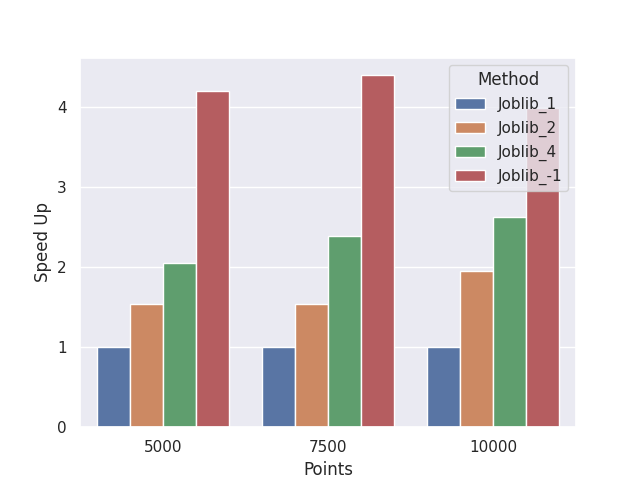
\includegraphics[scale=0.5]{../plots/JoblibSpeedUp.png}
\end{figure}

In Figure \ref{fig:numba}, we can observe the significant increase in speed-up achieved with Numba compared to Joblib. This improvement is more than linear due to the fact that Numba is compiled, eliminating the overhead associated with the Global Interpreter Lock (GIL) in Python.

\begin{figure}[H]
	\caption{Numba and Joblib speed up}
	\centering
	\label{fig:numba}
	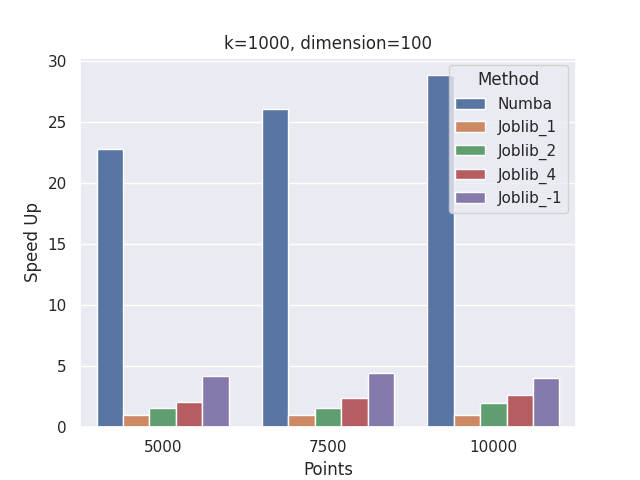
\includegraphics[scale=0.5]{../plots/numbaJoblibSpeedUp.png}
\end{figure}

{\small
	\bibliographystyle{ieee}
	\bibliography{egbib}
}

\end{document}
